\documentclass{article}
%=================Begin:Packages===================
\usepackage{graphicx}
%Please add your packages here
%=================End:Packages===================

%=================Begin:Macros===================
\newcommand{\Nom}{\ensuremath{\mathcal{N}}} % Set of nominators
\newcommand{\Val}{\ensuremath{\mathcal{V}}} % Set of elected validators
\newcommand{\nval}{\ensuremath{n_{val}}} % Number of validators to elect
\newcommand{\Can}{\ensuremath{\mathcal{C}}} %Set of candidate validators
\newcommand{\nom}{\ensuremath{}} % A nominator
\newcommand{\val}{\ensuremath{}} %A validator
\newcommand{\col}{\ensuremath{}} %A collator
\newcommand{\Par}{\ensuremath{P}} %A particilar parachain
\newcommand{\Col}{\ensuremath{\mathcal{C}}} %Set of collators
\newcommand{\slot}{\ensuremath{sl}} %slot number
\newcommand{\ep}{\ensuremath{e}} %epoch number
\newcommand{\lclock}{\ensuremath{\mathsf{clock}}} %local clock
\newcommand{\block}{\ensuremath{B}} % a block
\newcommand{\bchain}{\ensuremath{\bar{B}}} %blockchain
\newcommand{\D}{\ensuremath{\Delta}}
\newcommand{\skvrf}{\ensuremath{\mathsf{sk}^v}} %vrf secret key
\newcommand{\pkvrf}{\ensuremath{\mathsf{sk}^v}} %vrf public key

%OTHER NOTATIONS WITHOUT MACROS
%\Val_\Par -> Validator set for a particular parachain \par

%=================End:Macros=====================

%=================Begin:Definitions===================
%Please add you variable definitions here
%=================End:Definitions===================



\title{Overview of Polkadot Design}

\author{}

\begin{document}

\maketitle

\begin{abstract}
In this paper we describe the design components of the heterogenous multi-chain Polkadot.

We review the properties that Polkadot aims to achieve and go over all the components that are designed to achieve those properties.

\end{abstract}


\tableofcontents
\newpage
\section{Introduction}
Say something in line with: blockchain are valuable technologies because...

Currently there have been hundreds chains implemented in the wild for various functions.
(maybe a table with 10 famous but very different chains?)
Each one has different characteristics and their own security set up.

There is a need for a system that can connect this heterogenous chains.

Moreover, having multiple security set ups causes a split in the security these systems can provide.
Gathering all this security power and have a shared security system increases security substantially.


\subsection{System Overview}
- state machine
- data structures

\section{Glossary}



%\eray{
\begin{longtable}{p{.15\textwidth}p{.55\textwidth}p{.1\textwidth}p{.1\textwidth}} \label{t:time}
    \textbf{Name}  & \textbf{Description} & \textbf{Symbol} (plural)& \textbf{Def} \\
    \hline
    BABE & A mechanism to assign elected validators randomly to block production for a certain slot. && \ref{sec:babe} \\
    BABE Slot & A period for which a relay chain block can be produced. It's about 5 seconds. & \slot & \ref{sec:babe} \\
    Collator & Assist validators in block production. A set of collators is defined as \Col . & \col (\Col) & \ref{par:collators} \\
    DOT & The Polkadot native token. && \ref{sec:economics} \\
    Elected\newline- validators & A set of elected validators. & \Val & \\
    Epoch & A period for which randomness is generated by BABE. It's about 4 hours. & \ep & \\
    Era & A period for which a new validator set is decided. It's about 1 day. && \\
    Extrinsics & Input data supplied to the Relay Chain to transition states. && \ref{par:extrinsics} \\
    Fishermen & Monitors the network for misbehavior. && \ref{par:fishermen} \\
    Gossiping & Broadcast every newly received message to peers. && \ref{sec:gossiping} \\
    GRANDPA & Mechanism to finalize blocks. && \ref{sec:grandpa} \\
    GRANDPA\newline- Round & A state of the GRANDPA algorithm which leads to block finalisation. && \ref{sec:grandpa} \\
    Nominator & Stake-holding party who nominates validators to be elected. A set of nominators is defined as \Nom . & \nom (\Nom) & \ref{par:nominators} \\
    NPoS & \emph{Nominated Proof-of-Stake} - Polkadot's version of PoS, where nominated validators get elected to be able to produce blocks. && \ref{sec:validators} \\
    Parachain & Heterogeneous independent chain. & \Par & \\
    PJR & \emph{Proportional-Justified-Representation} - Ensures that validators represent as many nominator minorities as possible. && \ref{par:decentralization} \\
    %PoS & \emph{Proof-of-Stake} - Alternative to PoW, where parties vote with locked funds. && \ref{sec:validators} \\
    PoV & \emph{Proof-of-Validity} - Mechanism where a validator can verify a block without having its full state. && \ref{sec:parachainblockproduction} \\
    %PoW & \emph{Proof-of-Work} - Mechanism where parties vote with processing power. && \\
    Relay\newline- Chain & Ensures global consensus among parachains. && \ref{sec:relaychain} \\
    Runtime & The Wasm blob which contains the state transition functions, including other core operations required by Polkadot. && \ref{par:state_transition} \\
    Sentry\newline- nodes & Specialized proxy server which forward traffic to/from the validator. && \\
    Session & ?? && \\
    STVF & \emph{State-Transition-Validation-Function} - A function of the Runtime to verify the PoV. && \ref{sec:parachainblockproduction} \\
    Validator & The elected and highest in charge party who has a chance of being selected by BABE to produce a block. A set of candidate validators is defined as \Can . The number of validators to elect is defined as \nval . & \val (\Val)& \ref{par:validators} \\
    VRF & \emph{Verifiable-Random-Function} - Cryptographic function for determining elected validators for block production. && \ref{sec:babe} \\
    XCMP & A protocol that parachains use to send messages to each other. && \ref{sec:XCMP} \\
\caption{Glossary for Polkadot}
\end{longtable}
%}

%\alfonso{}{I think the table should contain more information. I would add a) possibly longer descriptions, b) a reference to the section that introduces them (and where we give an even longer description + its reason of being), and c) their lengths in seconds/minutes/hours, where we put a big note saying all lengths are tentative and subject to change considerably.}
%\alfonso{}{Also, we should either add "session" to the table, or remove all mentions of sessions. Simplifying could be a good idea, so maybe the latter?}
\section{Comparison with other multi-chain systems}\label{sec:comparison}
\paragraph{ETH2.0}

\subsubsection{Sidechains}
\paragraph{Cosmos} 

Much like Polkadot, Cosmos is a system designed to solve the blockchain interoperability problem that is fundamental to improve the scalability for the decentralized web. In this sense, there are surface similarities between the two systems. Hence, Cosmos consists of components which play similar roles and resemble the sub-components of Polkadot. For example, the Cosmos Hub is used to transfer messages between Comos' zones similarly to how the Polkadot Relay Chain oversees the passing of messages among Polkadot parachains.

There are however significant differences between the two systems. Most importantly, while the Polkadot system as a whole is a sharded state machine (See Section \ref{sec:relaychain}), Cosmos does not attempt to unify the state among the zones and so the state of individual zones is not reflected in the Hub's state. As the result, unlike Polkadot, Cosmos does not offer shared security among the zones. Consequently, the Cosmos cross-chain messages, are no longer trust-less. That is to say, that a receiver zone needs to fully trust the sender zone in order to act upon messages it receives from the sender. If one considers Cosmos system as a whole, including all zones in a similar way one analyses the Polkadot system, the security of such a system is equal to the security of the least secure zone. Similarly the security promise of Polkadot guarantees that validated parachain data are available at a later time for retrieval and audit (See Section \ref{sec:validity-and-availability}). In the case of Cosmos, the users are ought to trust the zone operators to keep the history of the chain state.

It is noteworthy that using the SPREE modules, Polkadot offers even stronger security than the shared security (See Section \ref{sec:spree}. When a parachain signs up for a SPREE module, Polkadot guarantees that certain XCMP messages received by that parachain are being processed by the pre-defined SPREE module set of code. No similar cross-zone trust framework is offered by the Cosmos system.

Another significant difference between Cosmos and Polkadot consists in the way the blocks are produced and finalized. In Polkadot, because all parachain states are strongly connected to relay chain states, the parachain can temporarily fork alongside the relay chain. This allows the block production to decouple from the finality logic. In this sense, the Polkadot blocks can be produced over unfinalized blocks and multiple blocks can be finalized at once. On the other hand, the Cosmos zone depends on the instant finality of the Hub's state to perform a cross-chain operation and therefore a delayed finalization halts the cross-zone operations.


\section{SPREE}

SPREE (Shared Protected Runtime Execution Enclaves) is a way for parachains to have shared code, and furthermore for the execution and state of that code to be sandboxed. From the paoint of view of parachain A, how much can it trust parachain B? Polkadot's shared security guarantees the correct execution of B's code with as much security as it does A's code. However, if we do not know B's code itself and even if we know the code now, maybe the governance mechanism of B can change the code and we do not trust that. This changes if we knew some of B's code, that it's governance did not have control of, and which could be sent messages by A. Then we would know how B's code would act on those messages if it was executed correctly and so shared security gives us the guarantees we need.

A SPREE module is a piece of code placed in the relay chain, that parachains can opt into. This code is part of that chains state transition validation function (STVF). The execution and state of this SPREE module are sandboxed away from the rest of the STVF's execution. SPREE modules on a remote chain can be addressed by XCMP. The distribution of messages received by a parachain would itself be controlled by a SPREE module (which would be compulsory for chains that want to use any SPREE modules). 

We expect that most messages sent by XCMP will be from a SPREE module on one chain to the same SPREE module on another chain. When SPREE modules are upgraded, which involves putting updated code on the relay chain and scheduling an update block number, it is upgraded on all parachains in their next blocks. This is done in such a way as to guarantee that messages sent by a version of the SPREE module one one chain to the same module on another are never recieved by past versions. Thus message formats for such messages do not need to be forward compatible and we do not need standards for these formats.

For an example of the security guarantees we get from SPREE, if A has a native token, the A token, what we would like is to be sure that parachain B could not mint this token. We could enforce this by A keeping an account for B in A's state. However if an account on B want's to send some A token to a third parachain C, then it would need to inform A. A SPREE module for tokens would allow this kind of token transfer without this accounting. The module on A would just send a message to the same module on B, sending the tokens to some account. B could then send them on to C and C to A in a similar way. The module itself would account for tokens in accounts on chain B, and Polkadot's shared security and the module's code would enforce that B could never mint A tokens. XCMP's guarantee that messages will be delivered and SPREE'S guarantee that they will be interpreted correctly mean that this can be done by just sending one message per transfer and is trust free. This has applications far beyond token transfer and means that trust minimising protocols are far easier to design.

Parts of SPREEs design and implementation have yet to be fully designed. Credit goes to u/Tawaren for the initial idea behind SPREE.
\section{Interoperability with External Chains}\label{sec:bridge}

\section{Properties}

 \subsection{Utility}

 The state machine of each parachain in Polkadot provides a utility to the system participants. It is ensured by state machines that interprets the willingness of a participant to pay for a transaction to be included.  Polkadot governance mechanism enables participants to decide what state machines should be included based on needs of participants.
 


 \subsection{Validity}
Each parachain in Polkadot has its own state transition function that defines how a parachain can move from the current state to a new state.   Validators in relay chain  know these functions and these functions let them  check whether a given state is valid or not.  In Polkadot, we have three levels of validity checks for each state of each parachain. The first-level check of a parachain state is executed by validators who are responsible for this parachain. These validators are called parachain validators and they shift from one parachain to another parachain periodically. The second level of check is executed by staked parties called fishermen which report to validators if they see any invalid state to receive some reward. And the last level of check is executed by randomly chosen validators after seeing no invalidity reports by parachain validators. These checks guarantee that it is almost impossible to have a finalized invalid state in the relay chain.

 \subsection{Finality}

 It is important to provide finality on a state of a parachain to preserve reliable communication in Polkadot so that parachains act by relying on the fact that the data provided by Polkadot related to other parachains will never change.  Polkadot provides the finality property via relay chain which is based on a heterogeneous consensus mechanism: provable consensus and probable consensus. The relay chain provides provable consensus with GRANDPA (GHOST-based Recursive ANcestor Deriving Prefix Agreement)  finality gadget. Validators are supposed to vote for a chain in GRANDPA  which has valid blocks (e.g., having valid states of parachains). The probable consensus is based on the block production mechanism of the relay chain that is called BABE (Blind Assignment for Blockchain Extension). BABE is a proof-of-stake based block production mechanism that privately and evenly assigns validators to produce blocks.

\subsection{Decentralization}

In some of the most popular blockchain projects, there are concerns of centralization of power. 
This centralization can be caused by several factors, such as 
a) a block-producer selection method where some minorities are over-represented or receive disproportionate power, or
b) an incentive mechanism that concentrates wealth or encourages cartel formation.
As we explain in the corresponding sections, our block-producer method (based on nominated proof-of-stake) 
as well as our incentive layer are particularly designed to fight centralization, 
and provide formally defined decentralization properties.


 \subsection{Availability}
The availability of messages in the relay chain is very critical because only available data can be validated. We call this data blob consisting of the parachain state and the proof of validity of that state. In Polkadot, we provide availability via erasure codes of blobs which are distributed to validators. Thus, when a validator needs a blob, he/she can contact with some subset of validators to construct the blob. We guarantee that an unavailable blob cannot be finalized in the relay chain since it cannot be validated.



%TODO IN FUTURE: We may need to add more detail about the following two properties
\subsection{Messaging Reliability} Polkadot provides message reliability by regulating and ordering what messages have been sent and received by which parachain or parathread. 

\subsection{Reasonable Size and Bandwidth} In Polkadot, the block size is selected carefully with respect to scalability and security.  

% How do we achieve them?

% Briefly breaking them down into components.

\section{Overview and Components}\label{sec:components}
%\begin{samepage}
Next, we summarise Polkadot functionality shortly for an overall picture and then continue to describe the individual components to show how to achieve that functionality.

Polkadot consists of a main chain called the relay chain and multiple sharded chains called parachains. The relay chain is maintained by validators that are selected through the NPoS scheme \ref{sec:validators} and is responsible for producing blocks of the  Relay Chain \ref{sec:babe} and keeping the state of all the parachains \ref{sec:relaychain}.
These validators need to vote on the consensus over all the parachains, see the consensus scheme \ref{sec:grandpa} for more details.
The security goal of Polkadot is to be Byzantine fault tolerant when the participants are rational (see \ref{sec:economics} for more detail on incentives and economics).
For parachains, there are additional actors called collators and fishermen that are responsible for parachain block production \ref{sec:parachainblockproduction} and reporting invalid parachain blocks respectively.
The parachain validators assigned to each parachain validate each parachain block and are responsible to keep it available, see \ref{sec:validity-and-availability}. Moreover, another feature of Polkadot is enabling interchain messaging among parachains, see \ref{sec:XCMP} for more details.
Furthermore, Polkadot has a decentralised governance scheme \ref{sec:governance} that can change any Polkadot design decisions and parameterisation.

%What do they achieve (refer to properties)?
\subsection{Validators (Network Maintainers)}
 \paragraph{Keys}

 \subsubsection{Validator selection}

 The Polkadot network selects a new set of validators at the beginning of each new era. We denote by \nval the target number of validators to be selected, which is in the order of hundreds or thousands and is proportional to the number of parachains. 

A validator node should satisfy certain requirements of speed, responsiveness and security. And DOT holder who is up to the task can submit their candidacy to become a validator, and they will be compensated for it, or slashed in the eventual case of a misconduct; see Section~\ref{sec:economics}. 

This setup leads to a multi-winner election problem based on approval ballots, where nominators have voting power proportional to their stake, and each nominator submits a list of validator candidates that she supports. A solution consists of a committee of $k$ validators, together with a distribution of each nominator's stake among the elected validators that she backs. We consider two objectives, both of which have been recently introduced in the literature of computational social choice. The first one is achieving the property of \emph{proportional justified representation} (PJR). The second objective, called \emph{maximin support}, is maximizing the minimum amount of stake that backs any elected validator. The former objective aligns with the notions of decentralization among validators as well as user satisfaction in the platform, while the latter aligns with the security level of the consensus protocol. 

We motivate the pursuit of these two objectives for the selection of validators in Polkadot as wells as any other decentralized protocol based on proof of stake with delegation. We also provide several constant-factor approximation algorithms for the maximin support objective, as well as a hardness result showing that these are, in a sense, best possible. Finally, we present a efficient algorithm which, when executed as a post-computation for any approximation algorithm for maximin support, ensures the PJR property while also preserving the approximation guarantee. Consequently, we provide the first efficient algorithms that simultaneously achieve PJR and constant-factor approximation guarantees for maximin support. 
\subsection{Parachains}
 \paragraph{Block Production}

 \paragraph{Validity and Availability}
 Once a block is created it is important that the parachain blob is available for a while.
 The naive solution for this would be broadcasting/gossip the parachain blobs to all, which is not a feasible option because the parachain blobs are big.
 We want to find an efficient solution to ensure parachain blobs from any recently created parachain block are available.

To this end we designed an availability scheme that uses erasure coding \cite{} to distribute the parachain PoV to all validators.
When any misbehaviour, unavailability particularly in relation to invalidity, is detected the PoV can be reconstructed from the distributed erasure coded pieces. 
 \paragraph{ICMP}

\subsection{Relay Chain State Machine}\label{sec:relaychain}

Formally, Polkadot is a replicated sharded state machine where shards are the parachains and the Polkadot relay chain is part of the protocol ensuring global consensus among all the parachains. Therefore, the Polkadot relay chain protocol, can itself be considered as a replicated state machine on its own. In this sense, this section describes the relay chain protocol by specifying the state machine governing the relay chain. To that end, we describe the relay chain state and the detail of state transition governed by transactions grouped in the relay chain blocks.

\paragraph{State:} The state is represented through the use of an \emph{associative array} data structure composed by a collection of $(key, value)$ pairs where each key is unique. There is no assumption on the format of the key or the value stored under it besides the fact that they both the key and the value need to be finite byte arrays.

A Merkle radix-16 tree keeps the Merkle hashes corresponding to the $(key, value)$ pairs stored in the relay chain state. They enable the identification of the current state using its root hash and provide efficient
proof of inclusion of a specific pair.

To keep the state size in control, the relay chain state is solely used to facilitate the relay chain operations such as staking and identifying validators. The Merkle Radix tree is not supposed to store any information regarding the internal operation of the parachains.

\paragraph{State transition: } \label{par:state_transition} Like any transaction-based transition system, Polkadot state changes via an executing ordered set of instructions. These instructions, traditionally known as transactions, are referred as extrinsics in Polkadot jargon. They cover any data provided from ``outside'' of the machine's state which can affect state transition. Polkadot relay chain is divided into two major components, namely the ``Runtime'' and the ``Runtime environment''. The execution logic of the state-transition function is mainly encapsulated in the Runtime while all other generic operations, commonly shared among modern blockchain-based replicated state machines, are embedded into the Runtime environment. In particular, the latter is in charge of network communication, block production and consensus engines.

Runtime functions are compiled into a Web assembly module and are stored as part of the state. The Runtime environment communicates the extrinsics with the Runtime and interacts with it to execute the state transition. In this way, the state transition logic itself can be upgraded as a part of the state transition.

\paragraph{Extrinsics:} \label{par:extrinsics}

Extrinsics are the input data supplied to the Polkadot relay-chain state machine to transition to new states. Extrinsics are needed to be stored into blocks of the relay chain in order to achieve consensus among the state machine replica. Extrinsics are divided into two broad categories namely transactions and inherents.

Transactions are signed and are gossiped around on the network between nodes. In contrast, inherents are not signed and are not gossiped individually but rather only when they are included in a block. The inherents in a block are assumed to be valid if a supermajority of validators assumes so. The timestamp is an example of inherent extrinsics which must be included in each Polkadot relay chain block.

Transactions on the relay chain are mainly concerned with the operation of the relay chain and Polkadot protocol as a whole, such as \texttt{set\_code}, \texttt{transfer}, \texttt{bond}, \texttt{validate}, \texttt{nominate}, \texttt{vote}.

Relay chain block producers listen to all transaction network messages. Upon receiving a transaction message, the transaction(s) are validated by the Runtime. The valid transactions then are arranged in a queue based on their priority and dependency and are considered for inclusion in future blocks accordingly.

\paragraph{Relay chain block format}
A typical relay chain block consists of a header and a body. The body simply consists of a list of extrinsics.

The header contains the \textit{hash of parent block}, \textit{block number}, the \textit{root of the state tree}, the \textit{root of the Merkle tree} resulting from arranging the extrinsics in such a tree and the \textit{digest}. The digest stores auxiliary information from the consensus engines which are required to validate the block and its origin as well as information helping light clients to validate the block without having access to the state storage.

\paragraph{Consensus:}

Polkadot Consensus protocol, similar to other replicated state machines, is responsible to guarantee liveness and safety. Liveness is the property that ensures that the state machine continues to collate and execute transactions. Safety, on the other hand, is the canonicalisation mechanism, or the means by which parties agree upon one of a number of possible, valid, histories and that ensures honest nodes do not agree on two conflicting states. This is also known as finality in the context of blockchains. These two properties ensure that valid transactions will eventually be included in the state transition
history and finalised.

Unlike the consensus architecture of many former blockchains, which builds a scalability bottleneck by tying the liveness and safety logic together, Polkadot architecture decouples the safety from the state-transition mechanism, a hybrid consensus model that separates block production from finality on those blocks (see Section \ref{sec:consensus}).

The block production layer of the consensus is to be fast and probabilistically safe. Block production randomly and secretly assigns the production of each block to a certain block producer to mitigate denial of service and eclipse attacks. The detail of Polkadot block production consensus sub-protocol is described in Section \ref{sec:babe}.

Simultaneously, the Polkadot execute a BFT-based consensus finality protocol which is tasked to observe possibly several incompatible, but likely valid, state transitions produced by the first layer and democratically finalise a canonical version as the valid history of the relay chain. Besides scalability, the choice of relay chain consensus protocol provides efficient absolute, in contrast to probabilistic, finality. That is, once a block is finalised, the canonical chain will always contain that block in the future. The finality subprotocol of Polkadot consensus is explained in Section
\ref{sec:grandpa}

\paragraph{Block Building}\label{sec:relaychainblockproduction}
In this section, we present a summary of various steps of relay chain operation which carried out by its validators. Validators of the being nominated and selected to produce and finalise a certain number of blocks. A priori, each validator privately knows the slot of the time during which it is supposed to produce a block and waits for its turn.

Meanwhile, transactions ranging from the validated parachain block hash, transfer, staking, nomination or slashing for protocol violation are submitted to the relay chain validators. The validators examine the validity of the transactions and store them in their transaction pool. Once the time slot during which the validator is expected to produce the block has arrived, the validator estimates the block which most likely represents the state which is going to be finalised by the finality protocol and set it as the current state of the relay chain. Then the validator selects valid transactions with fulfilled pre-requisite from the transaction pool, executes them and updates the state accordingly. The validator executes and collates as many transactions as the block capacity allows and attaches a cryptographic digest of the final stage of the relay chain after executing the selected transactions. Finally the validator signs and publishes the built block.

Upon receiving the new block, other validators examine that the producer's adherence to the protocol as well as the validity of included transactions and store the block in the \emph{block tree} which represents all possible candidates for a final state transition of the relay chain. 

Simultaneously, the set of validators votes on various branches of the block tree and prunes branches which conflict with the version agreed upon by the supermajority of the validators. In that way, they eventually agree on a canonical state of the relay chain.

\subsection{Consensus}\label{sec:consensus}

In this section, we explain the hybrid consensus protocol of Polkadot which consists of BABE: a block production mechanism of the relay chain that provides probabilistic finality and GRANDPA which provides provable, deterministic finality and works independently from BABE.  Informally probabilistic finality implies that after certain time passes, a block in the relay chain will be finalised with very high probability (close to 1) and deterministic finality implies a finalised block stays final forever. Furthermore provable finality means that we can prove to parties not actively involved in the consensus that a block is final.

We need provable finality to make bridges to chains outside Polkadot easier and for that we need Byzantine agreement. However the availability and validity scheme \ref{sec:availabilityandvalidity} may also require us to revert blocks, which would mean that getting Byzantine agreement on every block, as in Tendermint \cite{Tendermint} or Algorand \cite{ALGORAND}, would not be suitable. However, this should happen rarely as a lot of stake will be slashed when we do this. As a result, we want a scheme that generates blocks and optimistically executes them, but it may take some time to finalise them. Thus GRANDPA voters need to wait for assurances of availability and validity of a block before voting to finalise that block.
Even the speed at which we finalise blocks may vary - if we do not receive reports of invalidity and unavailability then we can finalise fast, but if we do then we may need to delay finality while we execute more involved checks. 

Because of the way Polkadot's messaging protocol (XCMP \ref{sec:icmp}) works, message passing speed is constrained by block time, but not by finality time. Thus if we delay finality but in the end do not revert, then message passing is still fast.

As a result of these requirements, we have chosen to separate the mechanisms for block production and finalising blocks as much as possible. In the next two sections, we describe the protocols BABE and GRANDPA that do these respectively.

%In our consensus protocols, we assume that a message sent by a validator arrives to other validators at most $\D$ times later where $\D$ is an unknown parameter. So, validators are in a partially synchronous network that guarantees  eventual delivery.
\subsubsection{Blind Assignment for Blockchain Extension (BABE)}
\label{sec:babe}

In Polkadot, we produce relay chain blocks using our Blind Assignment for Blockchain Extension protocol \eray{, abbreviated BABE}{(BABE)}. BABE assigns validators randomly to block production slots using  the randomness generated with blocks. These assignments are completely private until the assigned validators produce their blocks. Therefore, we use ``Blind Assignment'' in the protocol name. BABE is similar to Ouroboros Praos \cite{Praos} with some significant differences in the chain selection rule and timing assumptions.

In BABE, we may have slots without any \eray{assignment}{assinments,} which we call empty \eray{slot}{slots}. In order to fill the empty slots, we have \eray{}{a} secondary block production mechanism based on Aura \cite{aura} that assigns validators to slots publicly. We note that these blocks do not contribute \eray{}{to} the security of BABE since the best chain selection algorithm works as if Aura blocks do not exist and \eray{the randomness generation \eray{do}{does} not consider randomness in the Aura blocks.}{-comment:I didn't understand this sentence.-}

Here, we only describe BABE together with its security properties since Aura blocks \eray{is}{are} not the part of the security of BABE.

\paragraph{BABE:}

BABE \cite{babe} consists of \emph{epochs} ($e_1,e_2,...$) and each epoch consists of a number of sequential block production slots (\(e_i = \{sl^i_{1}, sl^i_{2},\ldots,sl^i_{t}\}\)) up to the bound  $R$.
Each validator knows in which slots that he is supposed to produce a block at the beginning of every epoch. When the time for their slot comes, they produce the block by proving that they are assigned \eray{}{to} this slot.

The blind assignment is based on the cryptographic primitive called verifiable random function (VRF) \cite{vrf} (See Section \ref{sec:session_keys}). 
A validator in an epoch $e_m$ where $m > 2$ does the following to learn if he is eligible to produce a block in slot $sl_i^m$: He retrieves the randomness $r_{m-2}$ generated two \eray{epoch}{epochs} before ($e_{m-2}$). Then, he runs the VRF with his secret key and the input:  randomness $r_{m-2}$ and the slot number $ sl_i^m $.  Validators in $e_1$ and $e_2$ use the randomness defined in the genesis block when they run the VRF with their secret key for the slots belonging $e_1$ and $e_2$. If the output of the VRF is less than the threshold $ \tau $, then the validator is the slot leader meaning that he is eligible to produce a block for this slot. We select $\tau$ considering the network delay \cite{babe}. 
When a validator produces a block, he adds the output of the VRF and its proof to the block which shows that his VRF output is less than $\tau$  in order to convince other validators that he has a right to produce a block in the corresponding slot. The validators always generate their blocks on top of the best chain.
The best chain selection rule in BABE says that ignore the Aura blocks and select the longest chain that includes the last finalized GRANDPA block. See Section \ref{sec:grandpa} for the details how blocks are finalized in GRANDPA.

The randomness of an epoch $e_m$ is generated by using the BABE blocks of the best chain that belongs to that epoch: Concatenate all  VRF values in BABE blocks that belongs to $e_m$  (let us assume  the concatenation is \(\rho\)). Then, compute the randomness in epoch $e_{m+1}$ as $r_{m} = H(m
||\rho)$ where $ H $ is a hash function. 

Validators run periodically the relative time algorithm described below to learn \eray{the}{-remove-} at what time a slot starts according to their local clocks.

\input{relativetime.tex}


\paragraph{\eray{-}{-remove-} Security Overview of BABE:} Garay et al. \cite{backbone} define the properties defined below in order to obtain a secure blockchain protocol. Informally, we can describe these properties as follows:

\begin{itemize}
	\item \emph{Common Prefix Property (CP) \eray{}{-comment: Isn't this CPP? How did you get CP as an abbreviation here?-}:} It ensures that the blocks which are $ k $-blocks before the last block of an honest validator's blockchain cannot be changed. We call  all unchangeable blocks  \emph{finalized} blocks. BABE satisfies CP property thanks to the honest super majority since malicious validators are selected for a slot probabilistically much less than the honest validators. It means that malicious validators \eray{does}{do} not have enough \eray{source}{sources} to construct another chain which does not include one of the finalized blocks.
	\item \emph{Chain Quality (CQ):} It ensures sufficient honest block contribution to any best chain owned by an honest party.	We guarantee even in the worst case where a network delay is maximum that there will be at least one honest block in the best chain during an epoch so that the randomness cannot be biased.
	\item \emph{Chain Growth (CG):} It guarantees a minimum growth between slots. Thanks to super majority of honest validators, malicious validators cannot prevent the growth of the best chain.	
	
	\item \emph{Chain Density (CD):} It ensures that in a sufficiently long portion of the best chain more than half of the blocks produced by honest validators. CQ and CD properties \eray{implies}{imply} this property \cite{Praos}.
\end{itemize}


\eray{Please see \cite{babe} for further details about BABE and  its security analysis.}{Further details about BABE and  its security analysis can be found in \cite{babe}.}


\subsubsection{GRANDPA} \label{sec:grandpa}


As mentioned above, we want a finalisation mechanism that is flexible and separated from block production, which is achieved by GRANDPA. The only modification to BABE required for it to work with GRANDPA is to change the fork-choice rule: instead of building on the longest chain, a validator producing a block should build on the longest chain including all blocks that it sees as finalised. GRANDPA can work with many different block production mechanisms and it should be possible to switch out BABE with another.

Intuitively GRANDPA is a Byzantine agreement protocol that works to agree on a chain, out of many possible forks, by following some simpler fork choice rule, which together with the block production mechanism would give probabilistic finality if GRANDPA itself stopped finalising blocks. We want to be able to agree on many blocks at once, in contrast to single-block Byzantine agreement protocols.

We assume that we can ask the fork choice rule for the best block given a particular block. 

The basic idea is that we want to agree by Byzantine agreement on the prefix of the chain that everyone agrees on. To make this more robust, we try to agree on the prefix of the chain that 2/3 of validators agree on.

\begin{figure}[h!]
  \centering
  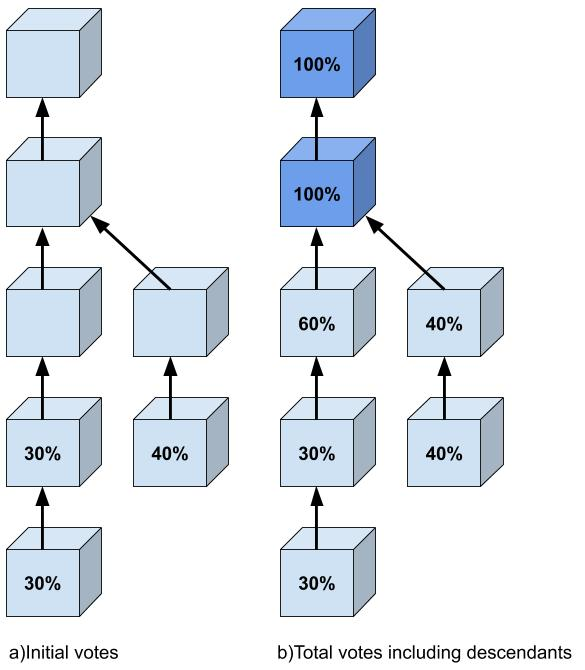
\includegraphics[width=0.7\textwidth]{images/Grandpa.jpg}
  \caption{GRANDPA votes and how they are aggregated.}
    \label{fig:grandpa}
\end{figure}

We make use of a GHOST on votes rule, much like Casper TFG \cite{CasperTFG} or some of the fork choice rules suggested for use with Casper FGG \cite{CasperFFG}. We use this rule inside what is structured like a more traditional Byzantine agreement protocol, to process votes. The 2/3 GHOST rule (pictured in Figure \ref{fig:grandpa})  works as follows. We have a set of votes, given by block hashes.  in which honest validators should not have more than one vote, and we take the head of the chain formed inductively as follows. We start with the genesis block and then include the child of that block that 2/3 of the voters voted for descendants of, as long as there is exactly one such child. The head of this chain is $g(V)$ where $V$ is the set of votes.

There are two voting phases in a round of GRANDPA, prevote and precommit. Firstly validators prevote on a best chain. Then they apply the 2/3-GHOST rule, $g$ to the set of prevotes $V$ they see and precommit $g(V)$. Then similarly they take the set of precommits $C$ they see and finalise $g(C)$.

To ensure safety, we ensure that all votes are descendants of any block that could possibly have been finalised in the last round. Nodes maintain an estimate of the the last block that could have been finalised in a round, which is calculated from the prevotes and precommits. Before starting a new round, a node waits until it sees enough precommits for it to be sure that no block later than or on a different to this round's estimate can be finalised. Then it ensures that it only prevote sand precommits in the next round to blocks that are descendants of the last round's estimate (which it keeps updating by listening to precommits from the last round). This ensures safety.

To ensure livness, we select one validator in rotation to be the primary. They start the round by broadcasting their estimate for the last round. Then when validators prevote, if the primary's block passes certain checks, among them that it is at least the validator's estimate, then it prevotes for the best chain including the primary's block. The idea here is that if the primary's block has not been finalised, then we make progress by finalising it. If it has not, and we all agree on the best chain including the last finalised block, which we should eventually if BABE works, then we now make progress by finalising that chain.
  



\subsection{Economics and Incentive Layer}\label{sec:economics}

Polkadot will have a native token called dot. Its various functions are described in this section.



\subsubsection{Staking rewards and inflation}

We start with a description of staking rewards, i.e.~payments to \emph{stakers} -- validators and nominators -- 
coming from the minting of new dots. 
Unlike other blockchain protocols, the amount of tokens in Polkadot will not be bounded by an absolute constant, but there will rather be a controlled yearly inflation rate. Indeed, recent research~\cite{chitra2019competitive} suggests that in a proof-of-stake based protocol the staking rewards must remain competitive, in order to maintain high staking rates and high security levels, so deflationary policies are advised against. 

In our design, dots minted for staking rewards are the main driver of inflation in the system. 
This is because Treasury (\autoref{sec:governance}), the only other mechanism that mints dots, 
is designed to closely match its expenditure to the average dot burning caused by transaction fees and slashings.
Thus, it is convenient to introduce our inflation model in this section as well. 
%We do not consider rewards coming from transaction fees, slashings, nor rewards to fishermen and other reporters of offenses; these will be analyzed in further sections. 

Recall from the description of the NPoS protocol (\autoref{sec:validators}) that both validators and nominators stake dots. 
They get paid roughly proportional to their stake, but can be slashed up to $100\%$ in case of a misconduct. 
Even though they are actively engaged for only one era%
\footnote{Recall that an era lasts approximately one day. See Table~\ref{t:time} in the Appendix.} 
at a time, they can continue to be engaged for an unlimited number of eras. 
During this period their stake is locked, meaning it cannot be spent, and it remains locked for several weeks after their last active era, to keep stakers liable to slashing even if an offense is detected late.

\paragraph{Staking rate, interest rate, inflation rate:} Let the staking rate be the total amount of dots 
currently staked by validators and nominators, divided by the current total dot supply. 
The stakers' average interest rate will be a function of the staking rate: 
if the staking rate dips below a certain target value selected by governance, 
the average interest rate is increased, thus incentivising more participation in NPoS, and vice versa. 
For instance, a target staking rate of $50\%$ could be selected as a middle ground between security and liquidity. 
If the stakers' average yearly interest rate is then set to $20\%$ at that level, 
we can expect the inflation rate to fluctuate closely around $50\%\times 20\% = 10\%$. 
Hence, by setting targets for the staking rate and stakers' interest rate, we also control the inflation rate. 
Following this principle, every era we adjust our estimate of the staking rate, 
and use it to compute the total amount of dots to be paid to stakers for that era.

\paragraph{Rewards across validator supports:} 
Once the total payout for the current era is computed, we need to establish how it is distributed.
Recall that the validator election protocol (\autoref{sec:validators}) partitions the active stake into 
\emph{validator supports}, where each validator support is composed of the full stake of one validator 
plus a fraction of the stake of its backing nominators, and this partition is made so as to make validator supports 
as high and evenly distributed as possible, hence ensuring security and decentralisation. 
A further incentive mechanism put in place to ensure decentralisation over time 
is paying validator supports equally for equal work, regardless of their stake. 
As a consequence, if a popular validator has a high support, its nominators will likely be paid less per staked dot 
than nominators backing a less popular validator. Hence, nominators will be incentivised to change their preferences 
over time in favour of less popular validators (with good reputation nonetheless), helping the system converge to the ideal case where all validator supports have equal stake.

In particular, we devise a point system in which validators accumulate points for each payable action performed, 
and at the end of each era validator slots are rewarded proportional to their points. 
This ensures that validators are always incentivized to maintain high performance and responsiveness. 
Payable actions in Polkadot include: a) validating a parachain block, 
b) producing a relay chain block in BABE, 
c) adding to a BABE block a reference to a previously unreferenced uncle block,%
\footnote{In the BABE protocol, at times two block producers may generate different blocks A and B at the same height, leading to a temporary fork in the relay chain. The fork will quickly be resolved and select one of the blocks, say A, as part of the main chain, while block B becomes an \emph{uncle} to all descendents of A. For security reasons, it is convenient to record and timestamp \emph{all} blocks produced, but since uncle blocks cannot be accessed via parent relations, we encourage block producers to explicitly add these references to the main chain.}
 and d) producing an uncle block.

\paragraph{Rewards within a validator slot:} As a nominator's stake is typically split among several validator supports, 
their payout in an era corresponds to the sum of their payouts relative to each of these supports. 
Within a validator support, the payment is as follows: 
First, the validator is paid a \emph{commission fee}, which is an amount intended to cover its operational costs. 
Then, the remainder is shared among all stakers -- both validator and nominators -- proportional to their stake. 
Thus, the validator receives two separate rewards: a fee for running a node, and a payout for staking. 
We remark that the commission fee is up to each validator to set, and must be publicly announced in advance. 
A higher fee translates to a higher total payout for the validator, and lower payouts to its nominators, 
so nominators will generally prefer to back validators will lower fees, and the market regulates itself in this regard. 
Validators who have built a strong reputation of reliability and performance 
will however be able to charge a higher commission fee, which is fair.

\medskip

We finalise the section with some observations on the incentives that our payout scheme is expected to cause on stakers. 
First, as validators are well remunerated and their number is limited, 
they have an incentive to ensure high backing levels from nominators to ensure getting elected, 
and thus they will value their reputation. Over time, we expect elections to be highly competitive 
and for elected validators to have strong track records of performance and reliability and large stake backings.
Second, even if payouts across different validator supports are independent of their stake, 
within a validator support each actor is paid proportional to their stake, 
so there is always an individual incentive to increase one's own stake. 
Finally, if a validator gains a particularly high level of backing, it can profit from it by either increasing 
its commission fee, which has the effect of raising its own reward at the risk of losing some nominations, 
or launching a new node as a validator candidate and splitting its backing among all its nodes. 
On this last point, we welcome operators with multiple validator nodes, 
and even aim to make their logistics simpler, so long as they disclose such correlations 
so that nominators can adjust their strategy accordingly.


\subsubsection{Relay-chain block limits and transaction fees}

\paragraph{Limits on resource usage:} We bound the amount of transactions that a relay-chain block can process, 
in order to a) ensure that each block can be processed efficiently even on less powerful nodes and avoid delays in block production; b) have guaranteed availability for a certain amount of high-priority, operational transactions such as misconduct reports, even when there is high network traffic; and c) limit the growth rate of the relay-chain state. 
In particular, we set block constraints on the following resources: on-chain byte-length, 
time and memory required to process the transactions, and increase in state storage.

We classify transactions into several types, according to their priority level and resource consumption profile. 
For each of these types we have run tests based on worst-case scenarios for state, and for different input arguments. 
From these tests, we establish conservative estimates on resource usage for each transaction, and we use these estimates to ensure that all constraints on resource usage are observed.

We also add an additional constraint on resources: we distinguish between regular and high-priority transactions, and only let regular transactions account for up to $75\%$ of each block resource limit. This is to ensure that each block has a guaranteed space for high-priority transactions of at least $25\%$ of resources.

\paragraph{Transaction fees:} We use the model described above to set the fee level of a transaction based on three parameters: its type, its on-chain length, and its expected resource usage. This fee differentiation is used to reflect the different costs that a transaction incurs on the network and on the state, and to encourage the processing of certain types of transactions over others. A fraction of every transaction fee is paid to the block producer, while another fraction goes to finance the Treasury (Section~\ref{sec:treasury}). We highlight that, for a block producer, the rewards coming from transaction fees may constitute only a small fraction of their overall revenue, just enough to incentivise inclusion on the block.

We also run an adaptive transaction fee schedule that reacts to the traffic level, and ensures that blocks are typically far from full, so that peaks of activity can be dealt with effectively and long inclusion times are rare. In particular, the fee of each transaction is multiplied by a parameter that evolves over time depending on the current network traffic. 

 

We make fees evolve slowly enough, so that the fee of any transaction can be predicted accurately within a frame of an hour. In particular, we do not intend for transaction fees to be the main source of income for stakers.



%\subsubsection{Slashing}

\subsection{Governance}\label{sec:governance}

Polkadot uses sophisticated mechanisms for Governance which allows it to evolve gracefully over time at the ultimate behest of its assembled stakeholders. A key and unfailing rule is that all changes to the protocol must be agreed upon by stake-weighted referendum -- the majority of stake always commands the network.

In order to make any changes to the network, the idea is to bring Dot holders together and administrate a network upgrade decision with the help of the Council (see Section \ref{s:council}). No matter whether the proposal is submitted by a Dot holder or by the Council, it will ultimately have to go through a referendum to let all Dot holders, weighted by stake, make the decision.

Each Dot holder in Polkadot has the right to: a) submit a proposal, b) endorse a public proposal to prioritise it in the referendum timetable, c) vote on all active referenda, d) become a candidate for a seat in the Council, and e) vote on candidates for the Council. In addition, any Dot holder may become a nominator or a validator candidate to participate in NPoS (see Section \ref{sec:validators}).

\subsubsection{Proposals and Referenda}

The core of the Polkadot logic is stored on-chain in an amorphous state-transition function and defined in a platform-neutral language: WebAssembly. Each proposal takes the form of a privileged function call in the runtime, that is able to modify the runtime code itself, achieving what would otherwise require a "hard fork". A proposal is then tabled and voted upon via referendum. 

Proposals can be started in one of several ways:
\begin{itemize}
\item a public proposal, which is submitted by any Dot holder;
\item a Council proposal, submitted by the Council;
\item a proposal submitted automatically as part of the enactment of a prior referendum, and
\item an emergency proposal submitted by the Technical Committee (Section~\ref{s:council}).
\end{itemize} 

Each proposal approved by referendum has an associated enactment delay, i.e.~a time interval between the referendum ending and the changes being enacted. For the first two types of proposals above this is a fixed interval, tentatively set to 28 days. For the third type, it can be set as desired. Emergency proposals deal with major problems with the network which need to be fast-tracked, and hence will have a shorter enactment delay. Having an enactment delay ensures a level of stability, as it gives all parties sufficient notice to adapt to the new changes. After this period, the call to the associated privileged function is automatically made.  

Any stakeholder can submit a \emph{public proposal} by depositing a fixed minimum amount of Dots, which stays locked for a certain period. If someone agrees with the proposal, they may deposit the same amount of tokens to endorse it. Public proposals are stored in a priority queue, and at regular intervals the proposal with the most endorsements gets tabled for a referendum. The locked tokens are released once the proposal is tabled.

\emph{Council proposals} are submitted by the Council, and are stored in a separate priority queue where the priorities are set at the Council's discretion.

%\alfonso{}{What happens with proposals automatically submitted by the enactment of a previous referendum -- do they go to the public-proposal queue or the Council-proposal queue, or a different queue? I don't know, we should ask Gavin.}

A \textbf{referendum} is a simple, inclusive, staked-weighted voting scheme. It has a fixed voting period, after which votes are tallied. Referenda are always binary: voting options are "aye", "nay", or abstaining entirely.

\paragraph{Timetables:} Every thirty days, a new proposal will be tabled and a referendum will come up for a vote. The proposal to be tabled is the top proposal from either the public-proposal queue or the Council-proposal queue, alternating between the two queues if both are non-empty. If both queues are empty, the slot is skipped in the referendum timetable. Multiple referenda cannot be active simultaneously, except for emergency referenda which follow a parallel timetable.

\paragraph{Vote counting:} Voting on referenda is open to all Dot holders with a voting power proportional to their stake, up to a possible vote multiplier which is awarded to some parties depending on their level of commitment to the system, as we explain now. A party must generally lock their tokens used for voting until at least the enactment delay period beyond the end of the referendum. This is in order to ensure that some minimal economic buy-in to the result is needed and to dissuade vote selling. It is possible to vote without locking at all, but in that case the voting power is a small fraction of a normal vote for the given stake. Conversely, Polkadot will offer \emph{voluntary extended locking}, that allows any party to increase their voting power by extending the period of time they are willing to lock up their tokens. This ensures that voters committed to the system long term, who are willing to increase their exposure to the decision of a referendum, have a greater say in the matter. 

\paragraph{Turnout biasing:} It may seem restrictive to force a full stakeholder-based process to do something as little as, say, nudging the block time down by $5\%$. However, without this rule the network would likely be unstable, as placing its control outside of the hands of stakeholders would create a misalignment that may lead to inaction or worse. However, by taking advantage of the fact that turnout is rarely $100\%$, we can effect different outcomes depending on the circumstances, crafting a balance of power between active and passive stakeholders. For example, simple voting systems typically introduce a notion of quorum, whereby a minimum amount of turnout must be reached before a change is passed. 

For public proposals, we generalise this notion into a "positive turnout bias", where additional turnout always makes change more likely, assuming the same yay-to-nay ratio. More specifically, in case of low turnout we favour the nay side, or status quo, by requiring a super-majority approval, and as turnout approaches $100\%$ the requirement dials down to majority-carries. This works on two principles: Firstly that the status quo tends to be safer than any change, and thus should have some bias towards it. Secondly that, like all means of empirical measurement, there is inevitably going to be some degree of inaccuracy and volatility over time, particularly when turnout is low -- a result could be $51\%-49\%$ one month and then change to $49\%-51\%$, and given the costs involved in enacting the changes of a proposal it is advantageous to ensure that a result would not likely flip shortly after enactment. 

On the other hand, for proposals submitted by the Council, referenda have no turnout bias and majority-carries is observed. The reasoning here is that proposals pre-approved by the Council are deemed safer and less likely to be reverted, so the previously mentioned issues are alleviated and we can let Dot holders freely decide on the matter. 

\begin{figure}[htb]
  \centering
  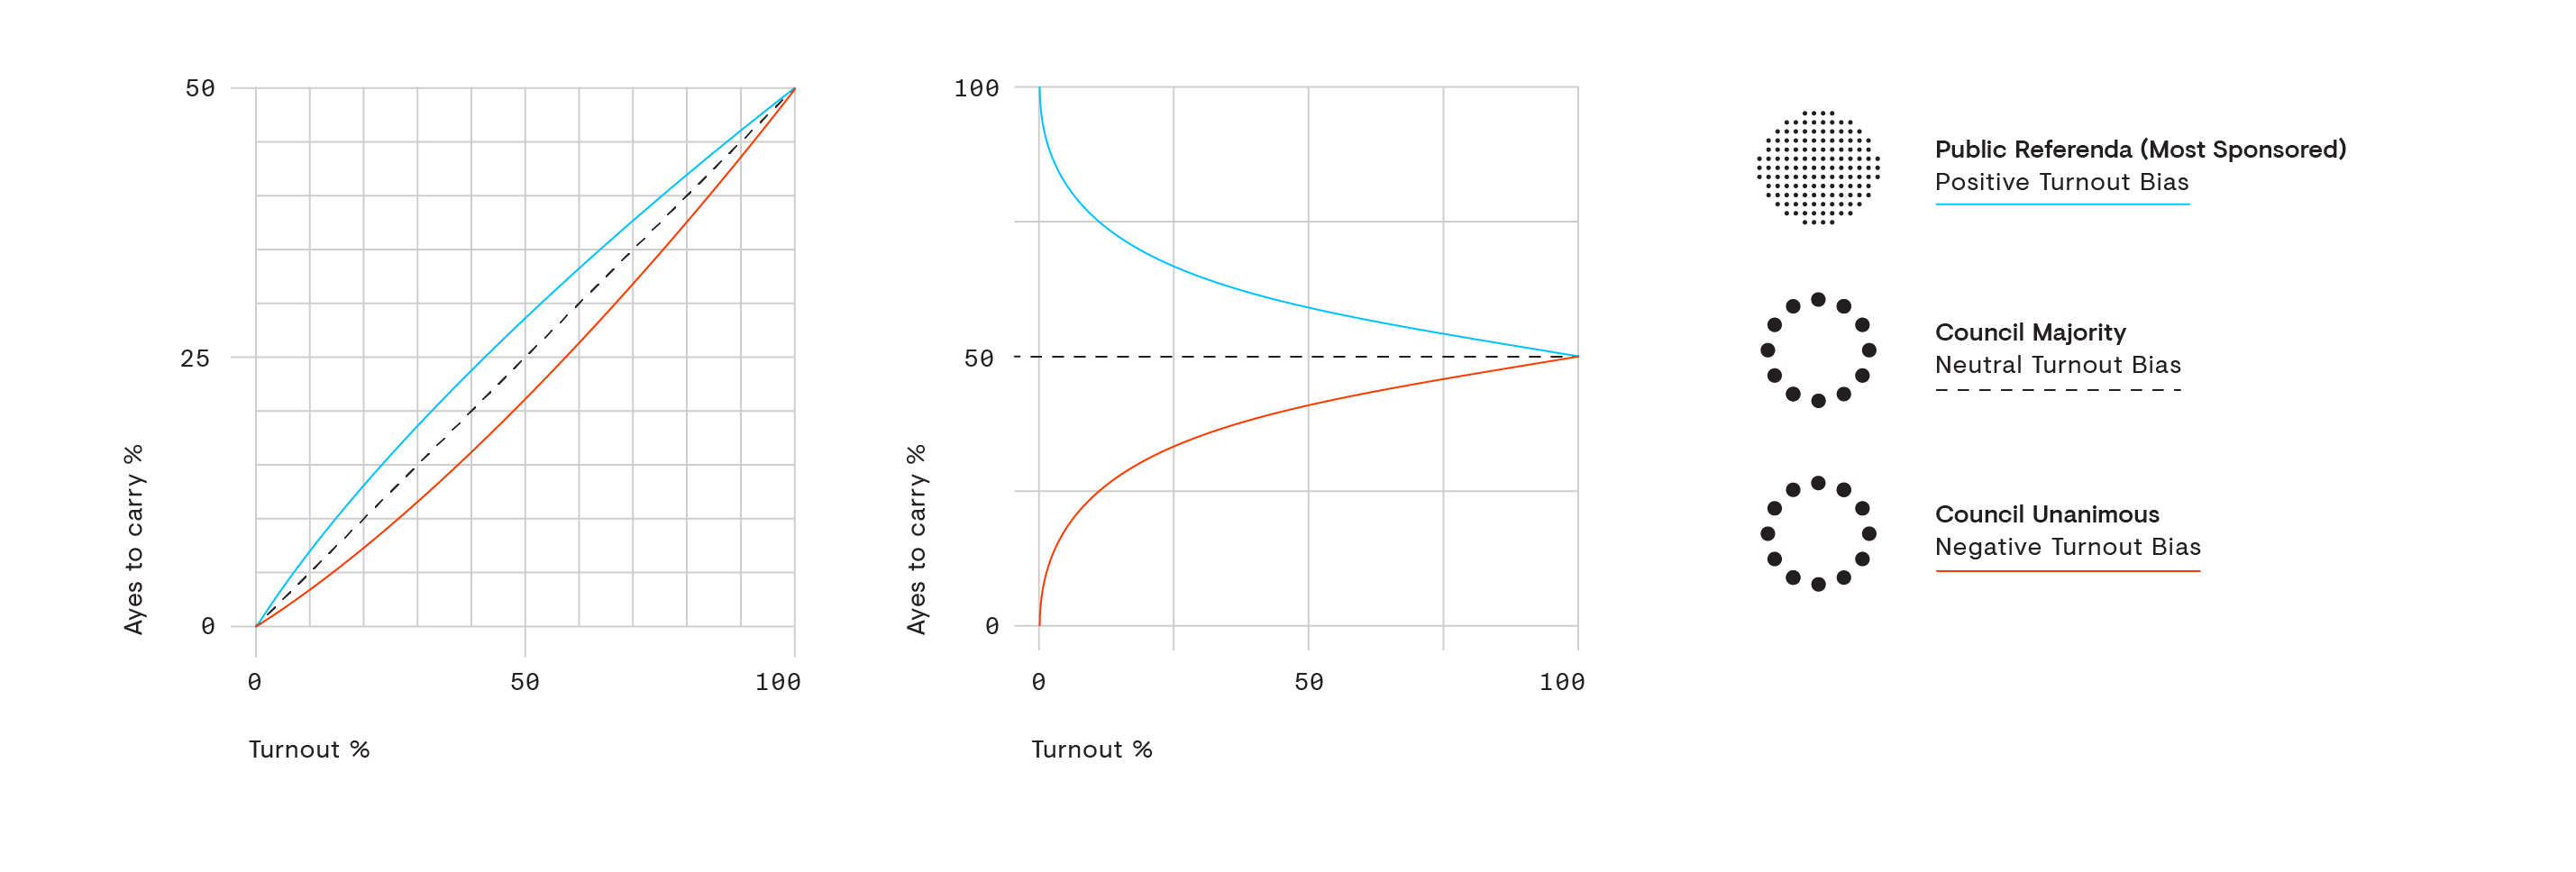
\includegraphics[width=1.1\textwidth]{images/Turnout-Bias.png}
  \caption{Adaptive turnout biasing (image credit: Ignasio Albero).}
    \label{fig:biasing}
\end{figure}

%\alfonso{}{Alfonso: Bill proposes that the biasing should be less severe. In particular for turnout values close to zero (which is what we observe in real life) the required percentage of ayes to carry stay, say, within 33 to 66\%, instead of going all the way to 0 or 100\%. I agree with him.}

Finally, in the exceptional case that a Council proposal receives unanimous support by all Council members, it will observe a "negative turnout bias". This is the symmetric opposite of the first case, where additional turnout always makes change less likely, we favour the yay side in case of low turnout by requiring a super-majority of nays to reject the proposal, and as turnout approaches $100\%$ the requirement dials down to majority-carries. See Figure~\ref{fig:biasing}.


\subsubsection{The Council and the Technical Committee}\label{s:council}

\textbf{The Council} is an entity comprising a number of actors each represented by an on-chain account. Its goals are to represent passive stakeholders, submit sensible and important proposals, and cancel uncontroversially dangerous or malicious proposals.

The Council will constantly review candidate proposals to deal with emerging issues in the system. A candidate proposal is officially backed by the Council -- and enters the queue of Council proposals -- only after it is approved by a strict majority of Council members, with no member exercising a veto. A candidate proposal can be vetoed only once; if, after a cool-down period, it is once more approved by a majority of Council members, it cannot be vetoed a second time. 

%\alfonso{}{The Council should have the capacity to change the bias of any proposal through majority voting or unanimity, even a public proposal. Is this the case now?}

As mentioned before, in the case that all members vote in favour, a Council proposal is consider uncontroversial and enjoys a special turnout bias that makes it more likely to be approved. 

Finally, Council members may vote to cancel any proposal, regardless of who submitted it, but their vote must be unanimous. Since unanimity is a high requirement, it is expected that this measure will only be used when it is an entirely uncontroversial move. This may function as a last resort if there is an issue found late in the day with a referendum's proposal such as a bug in the code of the runtime or a vulnerability  that the proposal would institute. If the cancellation is controversial enough that there is at least one dissenter, then it will be left to all Dot holders en masse to determine the fate of the proposal, with the registered Council cancellation votes serving as red flags so that voters pay special attention.

\paragraph{Electing Council members:} At Polkadot Genesis, there will be 6 to 12 seats in the Council, and an extra seat will be added every two weeks, ultimately settling at 24 seats.  All Council members have a fixed term of one year, and a member can be removed early only by referendum. 

All Dot holders are free to register their candidacy for the Council, and free to vote for any number of candidates, with a voting power proportional to their stake. A general election for the 24 Council seats will take place once a year. Much like the validator election problem in NPoS, this is a stake-weighted, multi-winner election problem based on approval ballots. We can thus solve it using the same algorithm we use for NPoS, which in particular offers the property of \emph{proportional justified representation}; see Section~\ref{sec:validators} for more details. This property guarantees that the elected Council will represent as many minorities as possible, thus ensuring that Governance stay decentralised and resistant to capture. Council members can be re-elected indefinitely, provided their approval remains high enough. 

\medskip

\textbf{The Technical Committee} is composed according to a single vote for each team that has successfully and independently implemented or formally specified the protocol in Polkadot, or in its canary network Kusama\footnote{http://kusama.network}. Teams may be added or removed by a simple majority of the Council. 

The Technical Committee is the last line of defence for the system. Its sole purpose is detecting present or imminent issues in the system such as bugs in the code or security vulnerabilities, and proposing and fast-tracking emergency referenda. An emergency proposal needs a simultaneous approval of at least three-quarters of the Council members and at least two-thirds of the Technical Committee members in order to be tabled. Once tabled, it is fast-tracked into a referendum that runs in parallel with the timetable of regular referenda, with a far shorter voting period, and a near-zero enactment period. The approval mechanics in this case are unchanged from what they would be otherwise, i.e.~either a simple majority or, in the case of a unanimous Council approval, a turnout-based bias for approval.

We highlight that for practical reasons the Technical Committee is not democratically elected, but in contrast it has an extremely reduced scope of action and no power to act unilaterally, as explained in the lines above. This mechanism is expected to suffice for non-contentious bug fixes and technical upgrades, but given the requirements imposed, may not be effective in the case of emergencies that have a tinge of political sensitivity or strategic importance to them. 
 
\subsubsection{Allocation of parachain slots}\label{s:pAllocation}

We use auctions to have a fair, transparent and permissionless parachain allocation procedure. 
Broadly speaking, parties interested in receiving a parachain slot participate in an auction with Dot-denominated bids. The party with the highest bid is declared as winner and is allocated a slot for a specific period of time, with its bid becoming a locked deposit that is released at the end of said period. The leasing cost of the slot thus corresponds to the opportunity cost of having this deposit locked. This Dot-denominated deposit also establishes the voting power of the parachain in Polkadot's governance.

Since implementing seal-bid auctions is difficult and in order to avoid bid sniping, we adopt a Candle auction \cite{Fuellbrunn:2012:CandleAuction} mechanism with a retroactively determined close. 
Going into detail, we plan to have an auction every few weeks, where in each auction four contiguous six-month slots are offered for lease. A bid can be made for any combination of one, two, three or four contiguous slots, for a total of ten possible time periods lasting 6, 12, 18 or 24 months. Once the auction starts, parties can post bids as transactions for any one of these ten periods, within a fixed window of time lasting several hours. A party is allowed to submit multiple bids, where a bid is registered only if a) it beats the current highest bid for the corresponding period, and b) the party does not become the provisional winner of two or more periods with gaps in between. For example, the winner of period $(1,2)$ -- constituted of the first two slots -- cannot bid on period $(4)$ -- the fourth slot -- until someone else overbids the former period. 

%A special data structure which allows us to 
We keep track of the provisional winners of all 10 periods at each point in time throughout the bidding time-window. Once this window is over, a public random number retroactively establishes a closing time within this window, thus also establishing a winner for each period.%
\footnote{More precisely, one of the blocks produced during the bidding time-window is selected by a public pseudo-random function, and all bids processes after that block are ignored. A cryptographic guarantee ensures that the pseudo-random function cannot be biased by any minority controlling less than 1/3 of the block production, with overwhelming probability.} %
The final winners correspond to the subset of non-overlapping periods with highest average bid per slot. For example, let us assume that at closing time we have the following winning bids: 75 Dots for period $(1,4)$, 30 Dots for period $(1,2)$, 90 Dots for period $(3,4)$, and 100 Dots for period $(2,3)$. In this example, set $[(1,2), (3,4)]$ has an average bid per slot of $(2\times 30 + 2\times 90)/4 = 60$, set $[(1,4)]$ has an average of $(4\times 75)/4 = 75$, and set $[(2,3)]$ has an average of $(0+2\times 100+0)/4=50$, so the final winner is set $[(1,4)]$. 

The stated goals of this design are to incentivise parties to bid early and avoid bid sniping, to give less funded projects a chance of winning a slot hence securing the decentralised nature of Polkadot, and to discourage grieving attacks by parties who raise the value of the winning bid with no intention of winning themselves.

\subsubsection{Treasury}\label{sec:treasury}

 The system needs to continually raise funds which we call the Treasury.
 These funds are used to pay for developers that provide software updates, apply any changes decided by referenda, adjust parameters, and generally keep the system running smoothly. Funds may also be used for further goals such as marketing activities, community events and outreach. This is ultimately controlled by all Dot holders via Governance and it will be the community and their collective imagination and judgment which really determines the course of the Treasury.

Funds for Treasury are raised in two ways:

\begin{enumerate}
\item by minting new tokens, leading to inflation, and
\item by channeling a fraction of transaction fees and of slashings.
\end{enumerate}

 
Notice that these methods to raise funds mimic the traditional ways that governments raise funds: by minting coins which leads to controlled inflation, and by collecting taxes and fines.
We could raise funds solely from minting new tokens, but we argue that it makes sense to redirect into Treasury some of the tokens from transaction fees and slashing that would otherwise be burned. By doing so, we reduce the amount of actual stake burning, and this gives us better control over the inflation rate, since stake burning leads to deflation and we cannot control the events that lead to burning. Furthermore, following an event that produced heavy stake slashing, the system is likely to need additional funds to develop software updates or new infrastructure that deal with an existing issue, or it might be decided by Governance to reimburse some of the slashed stake. Thus, it makes sense to have the slashed Dots available in Treasury, instead of burning them and having to mint more Dots soon thereafter.

\subsection{Cryptography}\label{sec:crypto}

In Polkadot, we necessarily distinguish among different permissions and functionalities with different keys and key types, respectively.  We roughly categorise these into account keys with which users interact and session keys that nodes manage without operator intervention beyond a certification process.

\subsubsection{Account keys}

Account keys have an associated balance of which portions can be {\em locked} to play roles in staking, resource rental, and governance, including waiting out a couple types of unlocking period.  We allow several locks of varying duration, both because these roles impose different restrictions, and for multiple unlocking periods running concurrently. 

We encourage active participation in all these roles, but they all require occasional signatures from accounts.  At the same time, account keys have better physical security when kept in inconvenient locations, like safety deposit boxes, which makes signing arduous.  We avoid this friction for users as follows.

Accounts that lock funds for staking are called {\em stash accounts}.  All stash accounts register a certificate on-chain that delegates all validator operation and nomination powers to some {\em controller account}, and also designates some {\em proxy key} for governance votes.  In this state, the controller and proxy accounts can sign for the stash account in staking and governance functions respectively, but not transfer fund.  

\smallskip

At present, we support both ed25519 \cite{ed25519} and schnorrkel/sr25519 \cite{schnorrkel} for account keys.  These are both Schnorr-like signatures implemented using the Ed25519 curve, so both offer extremely similar security.  We recommend ed25519 keys for users who require Hardware Security Module (HSM) support or other external key management solution, while schnorrkel/sr25519 provides more blockchain-friendly functionality like Hierarchical Deterministic Key Derivation (HDKD) and multi-signatures.  

In particular, schnorrkel/sr25519 uses the Ristretto implementation \cite{Ristretto} of Mike Hamburg's Decaf \cite[\S7]{Decaf}, which provide the 2-torsion free points of the Ed25519 curve as a prime order group.  Avoiding the cofactor like this means Ristretto makes implementing more complex protocols significantly safer.  We employ Blake2b for most conventional hashing in Polkadot, but schnorrkel/sr25519 itself uses STROBE128 \cite{STROBE}, which is based on Keccak-f(1600) and provides a hashing interface well suited to signatures and non-interactive zero-knowledge proofs (NIZKs).
% See https://github.com/w3f/schnorrkel/blob/master/annoucement.md for more detailed design notes.

\subsubsection{Session keys}\label{sec:session_keys}

Session keys each fill roughly one particular role in consensus or security.  As a rule, session keys gain authority only from a session certificate, signed by some controller key, that delegates appropriate stake.  

At any time, the controller key can pause or revoke this session certificate and/or issue replacement with new session keys.  All new session keys can be registered in advance, and most must be, so validators can cleanly transition to new hardware by issuing session certificates that only become valid after some future session.  We suggest using pause mechanism for emergency maintenance and using revocation if a session key might be compromised.  

We prefer if session keys remain tied to one physical machine because doing so minimises the risk of accidental equivocation.  We ask validator operators to issue session certificate using an RPC protocol, not to handle the session secret keys themselves.  

Almost all early proof-of-stake networks have a negligent public key infrastructure that encourages duplicating session secret keys across machines, and thus reduces security and leads to pointless slashing.
% TODO: I'd meant to cite this somewhere, but not sure where now.  It's easy to cite the slashing to part to cosmos.  Thoughts?

\smallskip

We impose no prior restrictions on the cryptography employed by specific components or their associated session keys types.\footnote{We always implement cryptography for polkadot in native code, not just because the runtime suffers from WASM's performance penalties, but because all of Polkadot's consensus protocols are partially implemented outside the runtime in Substrate modules.}

In BABE \ref{sec:babe}, validators use schnorrkel/sr25519 keys both for regular Schnorr signatures, as well as for a verifiable random function (VRF) based on NSEC5 \cite{NSEC5}.  

A VRF is the public-key analog of a pseudo-random function (PRF), aka cryptographic hash function with a distinguished key, such as many MACs.  We award block production slots when the block producer scores a low enough VRF output $\mathtt{VRF}_{\sk}(r_e || \mathtt{slot\_number} )$, so anyone with the VRF public keys can verify that blocks were produced in the correct slot, but only the block producers know their slots in advance via their VRF secret key.

As in \cite{Praos}, we provide a source of randomness $r_e$ for the VRF inputs by hashing together all VRF outputs form the previous session, which requires that BABE keys be registered at least two full epochs before being used.

We reduce VRF output malleability by hashing the signer's public key alongside the input, which dramatically improves security when used with HDKD.  We also hash the VRF input and output together when providing output used elsewhere, which improves composability when used as a random oracle in security proofs.  See the 2Hash-DH construction from Theorem 2 on page 32 in appendix C of \cite{Praos}.  

In GRANDPA \ref{sec:grandpa}, validators shall vote using BLS signatures, which supports convenient signature aggregation and select ZCash's BLS12-381 curve for performance.  There is a risk that BLS12-381 might drops significantly below 128 bits of security, due to number field sieve advancements.  If and when this happens, we expect upgrading GRANDPA to another curve to be straightforward. 
% https://mailarchive.ietf.org/arch/msg/cfrg/eAn3_8XpcG4R2VFhDtE_pomPo2Q

% TODO: ImOnline
% ref. https://github.com/paritytech/substrate/issues/3546

We treat libp2p's transport keys roughly like session keys too, but they include the transport keys for sentry nodes, not just for the validator itself.  As such, the operator interacts slightly more with these.

% As mentioned above, we permit controller keys to revoke session key validity of course, but controllers could pause operation for shorter periods.  We similarly permit controllers to register new session keys in advance, which enables a clean handover between validator machines.


\subsection{Networking}

%\end{samepage}

\section{Summary and Achieved Goals}
In this section we summarise Polkadot's components and describe what they aim to achieve. 

NPoS \ref{sec:validators} tries to ensure, under reasonable assumptions about the stakers, that every validator is well backed by stake. It gives an economic incentive to back validators equally. It also algorithmically tries to achieve this as much as possible given the nominator's votes if they are prepared to trust more than one validator with their stake.  This allows it to adapt to changing circumstances even when the votes themselves do not change.

If NPoS succeeds in making every validator well backed, the availability and validity scheme \ref{sec:validity-and-availability} then ensures, that any attack on the validity of Polkadot is expensive in expectation. That is, the entirety of Polkadot'd economic security backs every parachain. If each parachain is backed by 1/100th of the stake, then if we catch any attempt at validity ...

For this to work, we need to be able to revert the chain until we know with good probability that all parachains are correct. This means that we need to be able to reorganise the chain and for that the chain needs to be capable of forking.

Thus we use a block production mechanism, BABE \ref{sec:babe}, that while run by validators, has similar properties to proof-of-work chains. Specifically we can use the longest chain rule as part of our consensus, and that the next block producer is not known in advance.

On its own BABE would require us to wait a long time after a block is produced for finality, when we expect with high probability that a block would never be reverted. Sometimes slow finality is required, to deal with challenges to availability. Most of the time however we would prefer to finalise blocks much faster.  To finalise blocks we use GRANDPA \ref{sec:consensus}, a finality gadget that is cleanly separated from block production, which gives it the adaptiveness this design needs. 

If an account on one parachain sends tokens to another parachain, then XCMP \ref{sec:XCMP} ensures that this message is delivered correctly. It is sent at a speed which is not dependent on how long it takes to finalise blocks, which means that it needs to deal with the possibility of Polkadot forking. The parachain and XCMP logic ensure that a fork of the relay chain defines a consistent history of Polkadot and so that messages only arrive when they have been sent previously in the history defined by this fork.

If this uses a SPREE module then that ensures that so long as the parachains execute correctly then tokens can only be created and destroyed in an agreed upon way. In turn the correct execution of the chains code is guaranteed bu the availability and validity scheme. SPREE ensures that this code is correct as well, even though chains can change their own code.

Governance...


\section{Synopsis}\label{sec:summary}
The aim of this section is to describe the main functionality of Polkadot without going into details about the design considerations and reasoning.
% Please keep this 2 pages or less.

The Polkadot system consists of a single open collaborative decentralised network called the relay chain, that interacts with many other external chains run in parallel called \emph{parachains}. From a high-level perspective, parachains are clients of the relay chain, which provides a security service to these clients, including secure communication. That is the sole purpose of the relay chain; parachains are the entities providing application-level functionality, such as cryptocurrencies etc.

The internal details of parachains are not a concern of the relay chain; parachains need only adhere to the interface we specify. Some of these expectations are natural components of blockchains, hence the naming. However, other non-blockchain systems may also run as a Polkadot parachain as long as they satisfy the interface. This is described below: relevant parts are \uline{underlined}.

These aspects may be abbreviated as, \emph{Polkadot is a scalable heterogeneous multi-chain}.

\subsection{Security model}

We assume that parachains are running as external untrusted clients of the relay chain. As mentioned, it only deals with them via an interface and does not make assumptions about their internals. For example, internally they may be permissioned or open; if some internal users subvert the parachain, from Polkadot's viewpoint the entire parachain (as a single client entity) is malicious.

The Polkadot relay chain is designed to deal with a level of malicious behaviour internally, as a requirement of being an open decentralised network. Specific individual nodes are untrusted, but an indeterminable subset of nodes lower-bounded in size are trusted, and the protocol works to ensure that the relay chain externally as a whole is trustable. The details of these assumptions are covered in \nameref{sec:security_model}.
\subsection{Nodes and roles}

The Polkadot relay chain network consists of nodes and roles. Nodes are the network-level entities physically executing the Polkadot software, and roles are protocol-level entities performing a particular purpose. Nodes may perform multiple roles.

On the network level, the relay chain is open. Any node may run the software and participate as any of these types of nodes:

\begin{enumerate}
\item Light client - retrieves certain user-relevant data from the network. Availability is irrelevant - they don't perform a service for others.
\item Full node - retrieves all types of data, stores it long-term, and propagates it to others. Must be highly available.
  \begin{enumerate}
  \item \hyperref[sec:net_sentry]{Sentry node} - publicly-reachable full nodes that perform trusted proxying services for a private full node, run by the same operator.
  \end{enumerate}
\end{enumerate}

Beyond distributing data, nodes may perform certain protocol-level roles listed next. Some of these roles have restrictions and conditions associated with them:

\begin{enumerate}
\item Validator - performs the bulk of the security work. Must be a full node of the relay chain.
\item Nominator - stakeholder who uses this to select validators. Can be done from a light client.
\end{enumerate}

Parachains may decide their own internal network structure, \uline{but are expected to interact with Polkadot via the following roles}:

\begin{enumerate}
\item Collator\footnotemark[1] - collects and submits parachain data to the relay chain, subject to protocol rules depending on the current state of the relay chain, described below. They are chosen in a way defined by the parachain, and must be full nodes\footnotemark[2] of it.
\item Fishermen - performs additional security checks on the correct operation of the parachain, on behalf of the relay chain who supplies a reward. This role is self-assigned and reward-incentized, and must be a full node of the parachain.
\end{enumerate}

\footnotetext[1]{Validators are in some sense a collator of the relay chain network, in that they collect extrinsics (e.g. transactions) within the relay chain network. However we typically only refer to them as validators even when performing these tasks, and the term \emph{collator} is reserved for parachain collators only.}

\footnotetext[2]{A \emph{full node} of a parachain in the abstract sense for non-blockchain parachains, means that they participate in it to a sufficient degree that they can verify all data passing through it.}

\subsection{Protocol}

The Polkadot relay chain protocol, including interaction with parachains, works as follows.

\begin{enumerate}
\item For each parachain:

  \begin{enumerate}
    \item \uline{Collators watch the progress of the block-producing and consensus protocols}, (2) and (5) respectively below, e.g. by participating in the relay chain as a full node. Based on what they think is the relay chain block BR most likely to be finalised, they build on top of the latest parachain block (or other data) BC that would be finalised by BR.
    \item \uline{Collators sign data building on top of BC and submit it, possibly indirectly}, to the validators assigned to their parachain (\emph{parachain validators} for short), for inclusion in the relay chain. Ideally they should submit a unique one, to help performance.
    \item The parachain validators decide which data to support, and present this as a \emph{candidate} to the relay chain.
  \end{enumerate}

\item A block-producing validator collects candidates from all parachains, and puts this collection along with any recent relay chain extrinsics into a relay chain head block. For performance, this does not contain the full data from all parachains, but only metadata and partial data, including security-related metadata.

In the unfavourable case, this can result in forks, resolved later in (5). This subprotocol is designed so that even with forks, participants have an idea of the block most likely to be finalised, similar to Proof-of-Work protocols.

\item A subprotocol is run to ensure that the full data is indeed available, including and distributing it to various other relay-chain nodes.

\item Data submitted from a parachain might include indications that they are sending messages to another parachain, including metadata to facilitate this. This is now included on the relay chain head(s), so recipient parachains are aware of which new messages have been sent to them. \uline{They now retrieve the message bodies from the sending parachains}.

\item The relay chain votes on the block and finalises it, resolving any forks to a single head.

\end{enumerate}

% There is a small section on bridges in the Appendix, suggesting that it is just initial ideas at the moment. It can be summarised here later, once we turn it into a proper first-level section.

The rest of the paper expands on the above - roles next in \nameref{sec:preliminaries}, and protocol subcomponents in \nameref{sec:components}.

\bibliographystyle{plain}
%\bibliography{references,crypto}
\end{document}
